%%%%%%%%%%%%%%%%%%%%%%%%%%%%%%%%%%%%%%%%%
% Journal Article
% LaTeX Template
% Version 1.0 (25/8/12)
%
% This template has been downloaded from:
% http://www.LaTeXTemplates.com
%
% Original author:
% Frits Wenneker (http://www.howtotex.com)
%
% License:
% CC BY-NC-SA 3.0 (http://creativecommons.org/licenses/by-nc-sa/3.0/)
%
%%%%%%%%%%%%%%%%%%%%%%%%%%%%%%%%%%%%%%%%%

%----------------------------------------------------------------------------------------
%	PACKAGES AND OTHER DOCUMENT CONFIGURATIONS
%----------------------------------------------------------------------------------------

\documentclass[twoside]{article}
\usepackage{etex}
\usepackage{pgfplots}
\usepackage{comment}
\usepackage{cite} % Better citations
\usepackage{setspace}
\usepackage{mathtools}
\usepackage[sc]{mathpazo} % Use the Palatino font
\usepackage[T1]{fontenc} % Use 8-bit encoding that has 256 glyphs
\linespread{1.00} % Line spacing - Palatino needs more space between lines
\usepackage{microtype} % Slightly tweak font spacing for aesthetics
\usepackage{graphicx}
%\usepackage[hmarginratio=1:1,top=16mm,columnsep=20pt]{geometry} % Document margins
\newcommand{\bigO}{\ensuremath{\mathcal{O}}}
\usepackage[headsep=0.05in,scale=1.0,margin={0.5in,0.5in},columnsep=20pt]{geometry}
%\oddsidemargin 0.0in %%this makes the odd side margin go to the default of 1inch
%\evensidemargin 0.0in
%\headheight 0.5in
%\topmargin 0.5in
%\textheight 9.0in
%\textwidth 6.5in %%sets the textwidth to 6.5, which leaves 1 for the remaining right margin with 8 1/2X11inch paper 

\usepackage{multicol} % Used for the two-column layout of the document
%\usepackage{hyperref} % For hyperlinks in the PDF

\usepackage[hang, small,labelfont=bf,up,textfont=it,up]{caption} % Custom captions under/above floats in tables or figures
\usepackage{booktabs} % Horizontal rules in tables
\usepackage{float} % Required for tables and figures in the multi-column environment - they need to be placed in specific locations with the [H] (e.g. \begin{table}[H])
\usepackage{lettrine} % The lettrine is the first enlarged letter at the beginning of the text
\renewcommand{\LettrineTextFont}{\rmfamily}
\usepackage{paralist} % Used for the compactitem environment which makes bullet points with less space between them

\usepackage{abstract} % Allows abstract customization
\renewcommand{\abstractnamefont}{\normalfont\bfseries} % Set the "Abstract" text to bold
\renewcommand{\abstracttextfont}{\normalfont\small\itshape} % Set the abstract itself to small italic text

\pagestyle{plain} % no page numbers in footer
\usepackage{scalefnt} %scale font for title
\usepackage{titlesec} % Allows customization of titles
\usepackage{comment}	%Allows addition of comments
%\usepackage[small,compact]{titlesec}
\titleformat{\section}[block]{\large\scshape\centering{\Roman{section}.}}{}{1em}{} % Change the look of the section titles 

%----------------------------------------------------------------------------------------
%	TITLE SECTION
%----------------------------------------------------------------------------------------

%\title{\vspace{-15mm}\fontsize{20pt}{5pt}\selectfont\textbf{Experienced Search}} % Article title

%----------------------------------------------------------------------------------------

\begin{document}
%\title{\vspace{-20mm}{On-Line Recognition of Continuous Mouse Gesture Sequences}}
%\date{}
%\maketitle % Insert title
\scalefont{2}
\centerline{Recognition of Unistroke Gesture Sequences}
\normalsize

%----------------------------------------------------------------------------------------
%	ARTICLE CONTENTS
%----------------------------------------------------------------------------------------

\begin{multicols}{2} % Two-column layout throughout the main article text

\section{Problem Statement}
\lettrine[nindent=0em,lines=2]{G}esture recognition is a sizable research area,
due to the many uses and applications of gesture detection.
One important domain where gestures are frequently encountered is law
enforcement, where a significant concern is recognition of gang symbols in
graffiti and other forms of hand-written communication. The United States
Federal Bureau of Investigation's Safe Streets and Gang Unit commonly encounters
handwritten communication using custom gestures\cite{lyddane_donald_united_2006}. 

Inspired by this problem of gesture recognition, we focused our efforts on a
similar problem with common features. Our problem is recognition of a unistroke
gesture sequence, defined as a continuous stroke (unistroke) consisting of
multiple gestures defined \textit{a priori} (see Figure 1). In our opinion, this
problem description is analogous to identifying known gang symbols in grafitti
markings. An additional constraint is to use little to no training data, analogous to the
extremely small amount of evidence typically available to law enforcement officials.

%Problem addressed and its importance
%    ⁃    poor: does not mention problem or does not say why it is important
%    ⁃    acceptable: problem is tied to societal needs and backed up with reasons
%    ⁃    exceptional: succeeds in really convincing the reader (way beyond lip service)

%------------------------------------------------
\section{Related Work}
Yang et al \cite{yang_gesture_1994} present work on recognition of individual
gestures in unistroke and multistroke gesture sequences of digits by
constructing an exhaustive set of HMMs. They train HMMs to recognize continuous
gesture sequences defined \textit{a priori}, which is a deficient approach for
our problem. Robust individual gesture recognition systems exist, such as the
mouse gesture recognition system developed by
Tanguay\cite{tanguay_jr_hidden_1995}. However, the implementation is tailored to
individual gesture recognition. Additionally, the \$1 recognizer
\cite{wobbrock2007gestures} is a single gesture recognition system which works
with no training (the system has a built-in representative gesture training
set), but the primary deficiency is its inability to recognize gesture
sequences.
%------------------------------------------------
\section{Approach}
%Approach (What was done?)
%    ◦    poor: minimal description, hard to understand/replicate
%    ◦    acceptable: is specific about what was implemented and explains it well
%    ◦    exceptional: well written, clear explanations, reproducible: you care about the reader!
Recognizing a unistroke gesture sequence properly is difficult primarily due to
the nature of the problem, described in the literature as an ``inverse
perception problem'', which is an acknowledged ``hard problem''
\cite{pizlo_perception_2001}. An inverse perception problem, as
described by Pizlo, ``is about inferring the properties of the distal stimulus X
given the proximal stimulus Y'', and the problem is ``ill-conditioned''. A
feature of an ill-conditioned problem most relevant here is the possibility of
an infinite number of distal stimuli (intended gesture sequences) that produce
the proximal stimulus (the 2-D point representation of the gesture sequence).

We created a prototype gesture recognizer with two phases of operation: (1) a
training phase, in which the user selects a gesture and subsequently trains by
providing additional gesture \emph{templates}, and (2) a recognition phase, in
which the user draws a unistroke gesture sequence for subsequent recognition.
For the purposes of this study, and also for user convenience, we restrict the
maximum number of gestures in the sequence to 3, but the system can accept any
finite length input. A screenshot of the system in recognition mode is shown in the following figure:

\begin{figure}[H]
	\centering
	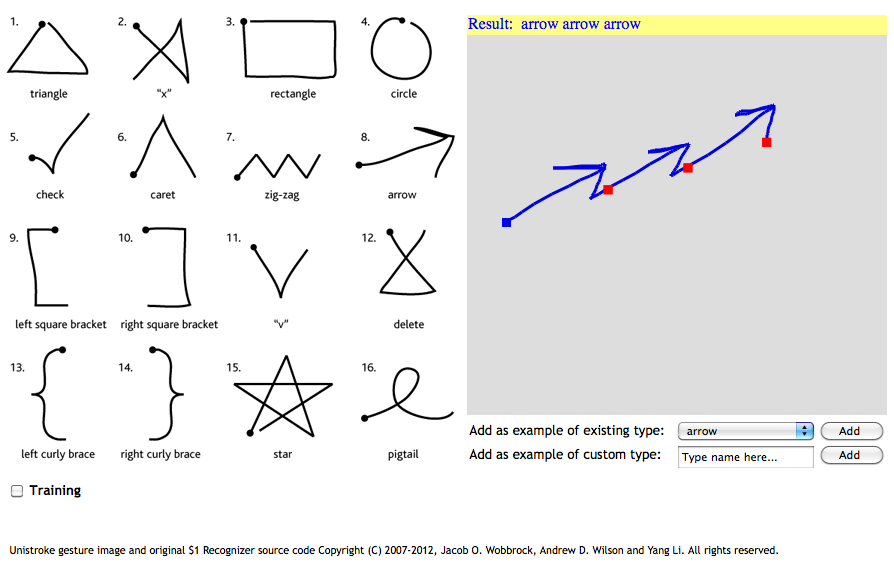
\includegraphics[height=5cm, width=8cm]{Images/GUI.png}
	\label{fig1}
	\caption{Recognition GUI}
\end{figure}
  
Our approach, at a high level, is estimating the \emph{visual affinity} of an 
input against multiple pre-existing templates. The first step
is to match each template against a portion of the input, thereby identifying a
segment of the input, and the remainder. The second step is to remove the first
gesture from the input sequence and iterate, searching for additional gestures.
A challenge to designing our approach was to account for variability in user
input. A feature of the inverse perception problem appears in the form
of segmentation ambiguity, as depicted in Figure 2.

\begin{figure}[H]
	\centering
	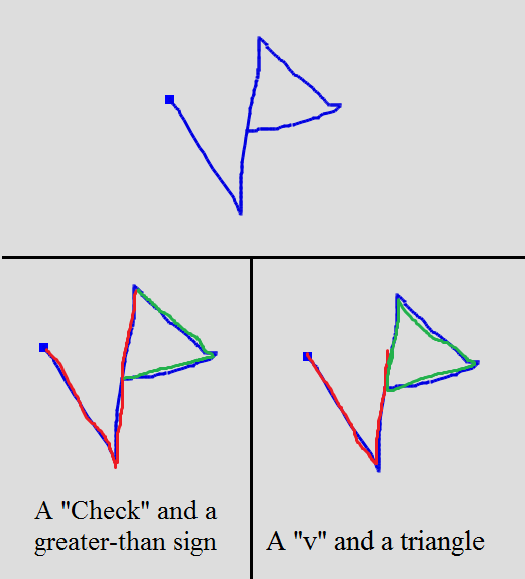
\includegraphics[height=4cm, width=5cm]{Images/Ambiguity1.png}
	\label{fig2}
	\caption{Ambiguity in gesture recognition}
\end{figure}

In the next section, we present details on our segmentation approach.

\subsection*{Segmentation}

During recognition, the user draws a unistroke gesture sequence, which is
recorded as an ordered list of $(x,y)$ coordinates. Each gesture template is
compared with the user's input. First, the template gesture is resampled to $64$
equidistant points in order to perform pointwise comparison against the user
input. Resampling is essential when comparing templates of \emph{individual}
gestures against the user input, which may contain \emph{one or more} individual
gestures. A fundamental insight into the problem that justifies our approach is
that a sequence of gestures is \emph{typically} (although not always) going to
have a longer 2-D path length than a single gesture. Next, the user's input is
also resampled, primarily to smooth out noise. We found that $64$ points was
high enough to retain the resolution necessary to disambiguate gestures and low
enough to be computationally inexpensive. Additionally, this number was
successfully used by the \$1 Recognizer\cite{wobbrock2007gestures}.

After resampling, the path length of the template is calculated and a threshold
is set at $90\%$ of the full path length. The purpose of the threshold is to
ensure that we don't require the full template data set to appear in the user's
input, which we felt was an intuitive and valid consideration (to see this,
simply consider the scenario for a gesture sequence of length $1$). The next
step is to calculate the corresponding number of points in the user's input
whose path length approximately equals the thresholded template path length.
Note that if $90\%$ of the full path length is longer than the path length of
the user input, the potential match is invalidated and skipped.

To determine a quantitative measure of the match, we score the segment pointwise
via dynamic time warping (see next section). At this point, we have a candidate
segment of user input with a score (lower indicates a better match) calculated
for a candidate point that separates the first identified gesture from the
remainder. However, it may be the case that a nearby point is actually a better
match (indicated by a smaller score). We test for the existence of a better
``segmentation point'' by searching both backward and forward in the user input,
repeatedly calculating the score. After the minimal score is computed, it is
stored for comparison against all other templates.

All of the gesture templates are scored in this manner and then sorted. The
smallest score is the best match, and this is marked as the identified gesture. An example
of the segmentation points for a unistroke gesture sequence is shown in Figure 1.

\subsection*{Dynamic Time Warping}

As mentioned above, our algorithm for scoring template gestures is dynamic time
warping (DTW). DTW is appropriate due to our need for flexible matching of
resampled input and template gestures. DTW ``warps" time to map each data point in
inputs X to the ``closest" matching point in input Y (as measured by the DTW distance
calculation). Recall that our inputs have differing numbers of sample points
(the template is resampled to $64$ points, but a segment of the user's input,
less than or equal to $64$ points, is chosen to compare with the template). For
our 2-D data, the appropriate distance metric is Euclidean distance. Using the
minimal cost of neighboring points (we compare the distance score for three ``nearby" points),
we map each point \emph{i} in input X to a nearest point \emph{j} in input Y.

%------------------------------------------------
\section{Evaluation}

%Evaluation (What were the results)
%    ◦    poor: just a qualitative assessment, no real results/numbers given
%    ◦    acceptable: qualitative as well as quantitative results, organized in tables and/or figures
%    ◦    exceptional: above and beyond in making the reader understand (not yet interpret) the results

The unique component of our system is our segmentation routine, which is
tightly coupled to (and dependent upon) the accuracy of the individual gesture
recognition algorithm (DTW). As a result, we evaluated our recognition system via three
metrics, which are, as whole, intended to provide insight into the system function.

\begin{enumerate}
\item Overall Accuracy: This is an all-or-nothing measure. For input sequence of
lengths 1, 2 or 3, we measure the percentage of trials in which the system
outputs both the correct number and correct identity of individual gestures (a perfect match).

\item
Segmentation Accuracy: For input sequence of lengths 1, 2 or 3, we measure the
percentage of trials in which the system outputs the correct \emph{number} of
gestures (regardless of correct identification of individual gestures).

\item Relaxed Accuracy: This is a relaxed version of Overall Accuracy relevant
only to gesture sequences of length 2 or 3, where we measure the number of
gestures in the output that actually appear in the input, accounting for order.
The purpose of this metric is to determine the percentage of trials where a
portion of the input was correctly segmented and identified.
For this metric, we count each gesture that was correctly identified, accounting
for gesture order. For example, if the input unistroke gesture sequence is
$check, star, \{$, and the system outputs $v, star, \{$, Relaxed Accuracy = 2, counting $star, \{$. Additionally, if
the sequence was identified as $v, star, caret, \{$, the Relaxed Accuracy = 2,
counting the $star$ and $\{$. The score assigned to a particular trial is:
\[
		Relaxed Accuracy = \frac{\text{Reported gestures in the input}}{\text{Total gestures in the input sequence}}
	\]
\end{enumerate}

We conducted a micro-study involving three participants and three recognition
phases. Each study participant chose 5 gestures out of the set of 16 to use for
the study. Then each participant drew 10 unistroke gesture sequence of lengths
1, 2, and 3 (for a total of 30) after three phases of training for each chosen gesture: 1 template, 3
templates, 5 templates, and 10 templates. We calculated the three aforementioned accuracy metrics for
the aggregate data. The results are shown in Tables 1,2 and 3 respectively.

\begin{table}[H]
  \centering
  \caption{Overall Accuracy}
    \begin{tabular}{rr}
    \toprule
    Sequence Length & Accuracy Rate \\
    \midrule
    1     & 57.5\% \\
    2     & 32.16\% \\
    3     & 25.72\% \\
    \bottomrule
    \end{tabular}%
  \label{tab:addlabel}%
\end{table}%

\begin{table}[H]
  \centering
  \caption{Segmentation Accuracy}
    \begin{tabular}{rr}
    \toprule
	Sequence Length & Segmentation Accuracy \\
    \midrule
    1     & 71.5\% \\
    2     & 71.5\% \\
    3     & 52.27\% \\
    \bottomrule
    \end{tabular}%
  \label{tab:addlabel}%
\end{table}%

\begin{table}[H]
  \centering
  \caption{Relaxed Accuracy}
    \begin{tabular}{rr}
    \toprule
    Sequence Length & Accuracy Rate \\
    \midrule
    2     & 56.19\% \\
    3     & 56.37\% \\
    \bottomrule
    \end{tabular}%
  \label{tab:addlabel}%
\end{table}%

Lastly, we calculated recognition accuracy for each training phase. Figure 3
displays Overall Accuracy (for sequences of length 1) and Relaxed Accuracy (for
sequences of lengths 2 and 3) for the different recognition phases.

\begin{figure}[H]
\centering
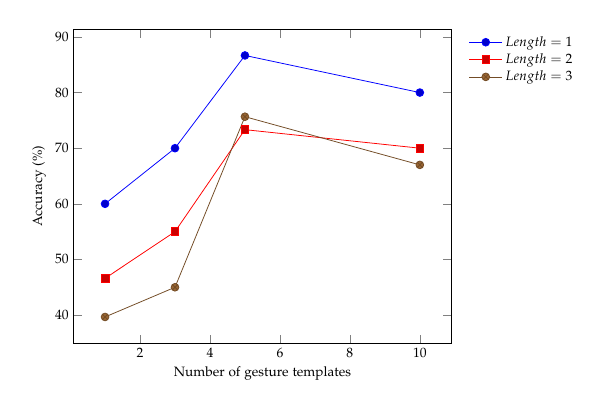
\begin{tikzpicture}[thick,scale=0.7, every node/.style={scale=0.7}]
    \begin{axis}[
	    legend pos= outer north east,
	    legend style={draw=none},
        xlabel=Number of gesture templates,
        ylabel=Accuracy (\%)
    ]
      \addplot plot coordinates {
        (1,     60)
        (3,    70)
        (5,   86.67)
        (10,   80)
    };

      \addplot plot coordinates {
        (1,     46.6)
        (3,    55)
        (5,   73.33)
        (10,   70)
    };

      \addplot plot coordinates {
        (1,     39.66)
        (3,    45)
        (5,   75.66)
        (10,   67)
    };
    
    \legend{$Length=1$\\$Length=2$\\$Length=3$\\}
    \end{axis}
\end{tikzpicture}	
	\caption{Recognition Rate Vs. \# of Gesture Templates}
	\label{fig3}
\end{figure}
%------------------------------------------------
\section{Discussion}

% Discussion (How to interpret the results)
%    ◦    poor: discusses and interprets the numbers and figures in the Evaluation Section
%    ◦    acceptable: in addition speculates about deeper reasons and/or insight into the algorithms that provides a better understanding to the reader
%    ◦    exceptional: additionally reflects on the entire project, discussing what you have learned, what you would change about what you did, and what possible additional work on this topic might be interesting

Tables 1, 2 and 3 reveal that our approach yields reasonable, but far from
perfect, results. The accuracy rate for sequence of length 1 (57.5\%) implies
DTW is a useful approach for comparing two data sets that vary in time.
This fact becomes clearer when we compare the DTW approach to the HMM approach
taken by Tanguay \cite{tanguay_jr_hidden_1995}, where he achieved a recognition
accuracy of $50-60\%$ on lower-case English alphabet letters after extensive
training. Note that the accuracy is lower for our problem than for the
simplified problem of 1-to-1 gesture template matching due to the ambiguity
introduced by a gesture sequence. In training phase, where only sequences of
length 1 are allowed, DTW excels at labeling the input correctly.

Table 1 shows a drop-off in accuracy as the sequence length increases. This
drop-off indicates a fundamental shortcoming in our approach: improper
recognition of a gesture is concomitant with improper segmentation of the
gesture sequence, leading to misrecognition of subsequent gestures. Yang et al
\cite{yang_gesture_1994} report a nearly perfect recognition rate of up to
99.78\% for sequences (only digits) of length 2. The difference in approach (reflecting
the difference in the objectives of problem statements), is a key consideration when comparing these
numbers. Yang et al train Hidden Markov models for both individual gestures as
well as gesture sequences. It is clear that training on gesture sequences
should yield significantly improved recognition rates.

Table 2 shows the percentage of trials that were correctly segmented into the
correct number of gestures. Note that, for each length, the trials in which
complete recognition was achieved (table 1) are a subset of the trials in which
the correct number of gestures was identified (table 2). As a result, one can
conclude that the difference in Overall Accuracy as compared to Segmentation
Accuracy is due to incorrect recognition of individual gestures. A more robust
technique for individual gesture recognition may significantly boost the
Overall Accuracy.

The Relaxed Accuracy results in Table 3 can be compared with the corresponding
Overall Accuracy results in Table 1. The increase in recognition accuracy
indicates that the system ``recovers" after a gesture is incorrectly identified.
This is noteworthy primarily because it implies that additionally training
intended specifically to address gesture ambiguity (including ambiguity with the
11 gestures the user did not choose) may significantly increase Overall
Accuracy.

Figure 3 clearly indicates that additional training increases both Overall
Accuracy and Relaxed Accuracy metrics. Importantly, ``excessive'' training may
lead to incorrect recognition due to the ``confusion" caused by having too many
variations of an individual gesture; put another way, too many templates
\emph{adds} ambiguity (``overfitting'').


We learned a great deal during this project. Most importantly, we significantly constrained
ourselves by training only on individual gestures. A key insight is that had we relaxed 
the problem (and as a result our objective) to also train on gesture sequences, 
it would have allowed us to determine the features 
that indicate a segmentation point, such as a slight pause between 
gestures in a gesture sequence (which we observed during the study). Thus,
having knowledge about the transition between gestures in a gesture sequence would have
helped us to dis-ambiguate potential gesture segmentation choices.

Reflecting upon the nature of the inverse perception problem, we hypothesize
that the problem is defined by identification of a hidden state (the intended
gesture sequence) corresponding to the ``distal stimulus X'' and observed via
``proximal stimulus Y''. Phrased in this manner,  Hidden Markov Models are ideal technique
to tackle this problem. Although HMMs require a larger training period, potential future work
could be to train HMMs on individual gestures and construct HMMs for all possible permutations
of gestures (i.e any gesture sequence) by simply chaining the already trained HMMs; this could lead to
better recognition rates at the expensive of time and computation power.
%----------------------------------------------------------------------------------------
\section{References}

\begin{spacing}{0.9}
%\scalefont{0.9}
\bibliographystyle{unsrt}	
%\bibliography{myrefs}
\begingroup
\renewcommand{\section}[2]{}%
\bibliography{myrefs}
\endgroup
\end{spacing}
%\normalsize

\end{multicols}
\end{document}

%	Member #1: Justin Permar - GT ID:902931271
%	Member #2: Arvind Krishnaa Jagannathan - GT ID: 902891874
%